\chapter{Approaching through neural data analysis}\label{cha:appr-thro-nda}

Based on the motivation elaborated in \autoref{cha:brain-as-complex},
we believe multi-scale and cross-scale analysis of neural data is one of the important aspect of neural data analysis from the complex systems prospective toward the brain
and indeed is one of the apertures through which,
we can seek for  the complementary approaches mentioned in \autoref{sec:toward-neur-insp}.
In this chapter, after further elaboration on the need for multi-scale and cross-scale analysis of neural data,
very briefly we discuss some of the relevant cross-scale neural data 
analysis methodologies and then introduce two novel methodologies that has been developed as part of this thesis.

\section{Necessity of investigating across scales}\label{sec:necess-invest-across}

As it was briefly discussed in \autoref{sec:toward-neur-insp},
understanding behavior in a system whose components  are neither behaving completely independent nor completely coherent, 
requires investigation \emph{across scales} \cite{bar-yamWhyComplexityDifferent2017,einevollScientificCaseBrain2019}.
Certainly, the brain is a prominent example of such systems \cite{einevollScientificCaseBrain2019}.
Perhaps the most intuitive aspect of the brain which demonstrates this point is its oscillatory dynamics.
As \citeAYt{chialvoEmergentComplexNeural2010c} pointed out, 
\begin{displayquote}\textsl{
    ``Recent work on brain rhythms at small and large brain scales showed that spontaneous healthy brain dynamics is not composed by completely random activity patterns or by periodic oscillations\cite{buzsakiRhythmsBrain2011}''.
  }
\end{displayquote}


In order to investigate the brain across scales,
first we need to clarify what is considered as the scale.
In this thesis, we refer to different \emph{levels of organization} as scales.
Brain is organized in different \emph{levels}
(\autoref{fig:levelOfOrg}).

% figure
\begin{figure}[h]
  \centering
  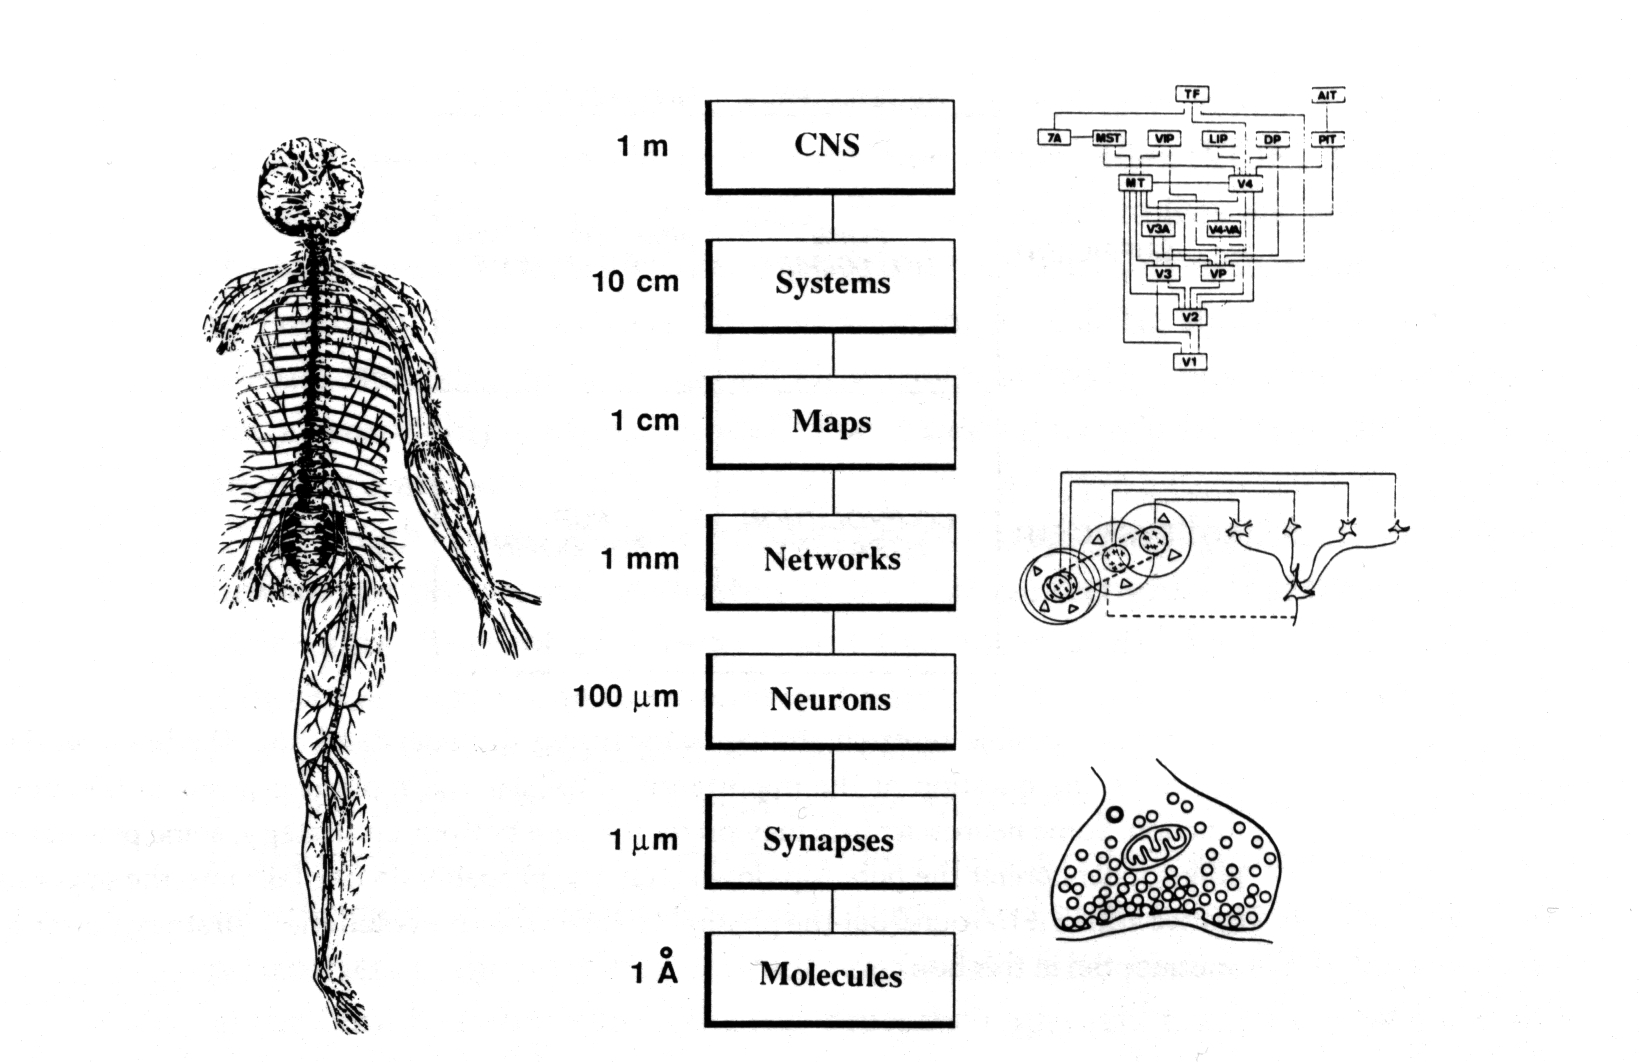
\includegraphics[width = \linewidth]{gfx/churchlan1988pcn_fig1.png}
  \caption{\textbf{Schematic depiction of levels of organization}\\
    Demonstrate extremely variable spatial scales at which anatomical organizations can be identified.
    Icons to the right represent structures at distinct levels:
    (top)
    a subset of visual areas in visual cortex;
    (middle)
    a network model of how ganglion cells could be connected to simple cells in visual cortex,
    and (bottom)
    a chemical synapse.
    Figure is adopted from \citet{churchlandPerspectivesCognitiveNeuroscience1988} with permission.}
  \label{fig:levelOfOrg}
\end{figure}
These levels range from scale of molecules all the way to large scale brain networks
\cite[Chapter 1]{churchlandComputationalBrain1992}.
Different phenomenon might primarily be explained in a limited range of these levels.
For instance, synaptic transmission, which is a basic form of communication in the brain, occurs at fairly small spatial scales, \ie level of molecules, synapses, and neurons.
Nevertheless, certain processes involve a broad range of levels. %\emph{levels}.
For instance in memory consolidation,
processes from gene expressions at the level of dendrites are involved,
all the way to larger-scale network \textbf{re}organization.
Therefore, one expects that process happening at different levels of organization to be related to each other.
It is worth to mention that, our understanding (especially from a theoretical perspective)
should be consistent across the levels of organization.
As elegantly described in \citet[Chapter 1]{churchlandComputationalBrain1992}:
% 
\begin{displayquote}\textsl{
    ``... the theories on one level must mesh with the theories of levels both
    higher and lower, because an inconsistency or a lacuna somewhere in the tale
    means that some phenomenon has been misunderstood.
    After all, brains are assemblies of cells, and something would be seriously amiss if neurons under
    one description had properties incompatible with the same neurons under
    another description.''
  }
\end{displayquote}


Indeed, there are various empirical evidence on predictions across scales and relationships between scales:
From single neurons to microcircuits \cite{raschInferringSpikeTrains2008a,raschNeuronsCircuitsLinear2009},
from microcircuits to a single brain area \cite{liBurstSpikingSingle2009a},
from a single area to the whole brain \cite{schwalmCortexwideBOLDFMRI2017,zerbiRapidReconfigurationFunctional2019}.
In some cases, the cross-scale coupling is closely and causally related to a specific function,
such as global state changes that have been shown in a study by \citet{liBurstSpikingSingle2009a}.
They showed that burst spiking of a single
cortical neuron in somatosensory cortex can induce a global switch between the slow-wave sleep and Rapid-Eye-Movement (REM) sleep.
In some cases, cross-scale relationships are even mechanistically interpretable as well.
For instance, it has been demonstrated that spiking probability can be modulated by the underlying network oscillation.
Network oscillations modulate the membrane potential of the neuron and that leads to the different levels of excitability for the given neuron.
Depending on the phase of the underlying oscillation, this can lead to a higher or lower probability of spiking activity \cite{volgushevLongrangeCorrelationMembrane2011,hasenstaubInhibitoryPostsynapticPotentials2005}.
Based on these simple mechanisms, \emph{coordination by oscillation} has been hypothesized,
and this lends support to various cognitive functions such as attention. 
The hypothesis of ``Coordination by oscillation'' proposes that network
oscillations modulate differently the excitability of several target populations,
such that a sender population can emit messages during the window of time for which a selected target is active, 
while unselected targets are silenced
\citep{friesRhythmsCognitionCommunication2015,womelsdorfModulationNeuronalInteractions2007a,friesMechanismCognitiveDynamics2005}.
Overall, I believe, considering \emph{two successive scales simultaneously},
is a principled approach for understanding collective or coordinated organizations in neural systems.
Furthermore, as mentioned in  \autoref{sec:toward-neur-insp} this approach is also justified by empirical evidence.


Investigating across scales can also be motivated from a more abstract 
(and perhaps more fundamental) perspectives:
In dynamical systems with non-linear interaction there are various examples where
activity in different scales are related \cite{levanquyenBrainwebCrossscaleInteractions2011}.
One example for such non-linear dynamical systems is the Kuramoto model.
As described briefly in \autoref{sec:complex-systems},
Kuramoto model describes a system of multiple coupled oscillators
\cite{kuramotoSelfentrainmentPopulationCoupled1975,kuramotoChemicalOscillationsWaves2003} 
(for an integrative review see \cite{acebronKuramotoModelSimple2005}).
In this model, the activity of individual oscillators is related to quantities pertaining to the average or mean-field activity of the system as a whole.
More precisely, the phase of an individual oscillator can be related to the mean phase of oscillators and their phase coherence.
Such core ideas from the theory of dynamical systems went beyond mere conceptual connections,
but also inspired unifying formulations for neural oscillations in the brain (\eg see \cite{breakspearGenerativeModelsCortical2010}).
For more detailed elaboration on motivations from the theory of dynamical systems for cross scales investigation of the brain see works of Le Van Quyen and colleagues
\cite{levanquyenExploringNonlinearDynamics2003,levanquyenDisentanglingDynamicCore00,levanquyenBrainwebCrossscaleInteractions2011}.

The other abstract motivation for investigation across scales is the nature of computation in the brain.
The brain is a naturally evolved biological information processing system.
Therefore, the computational strategies or solutions served by the brain can be quite different from engineered information processing systems \cite[Chapter 1]{churchlandComputationalBrain1992}\cite{douglasRecurrentNeuronalCircuits2007}.
The main difference between commonly engineered information processing systems and natural information processing systems is that the latter is constrained by the existing form of evolving organisms.
As elaborately framed by \citet[Chapter 1]{churchlandComputationalBrain1992}:
\begin{displayquote}\textsl{
    ``Evolutionary modifications are
    always made within the context of an organization and architecture that are
    already in place. Quite simply, Nature is not an intelligent engineer. It cannot
    dismantle the existing configuration and start from scratch with a preferred
    design or preferred materials.
    It cannot mull the environmental conditions and construct an optimal device.''
  }
\end{displayquote}
Furthermore, there are other aspects that need to be taken into account in the process of thinking about the solution chosen by the brain.
For instance,
humans/animals are constrained by the response time (they need to be fast enough) to be able to survive in their natural environment.
Finding the solution for the required computation is expected to happen in a few hundred milliseconds.
This becomes even more puzzling if we take into account the computational machinery in the brain that is orders of magnitude slower than artificial information processing systems.
Events in neurons happen in range of milisecond ($10^{-3}$)
as opposed to  nano second ($10^{-9}$) in electronic computers \cite{douglasRecurrentNeuronalCircuits2007}.
Other such examples are, spatial constrains (limitation by available space), energy consumption, and metabolism
\cite[Chapter 1]{churchlandComputationalBrain1992}).
\textbf{All being said to minimize the surprise of mentioning novel proposals (in the following) on brain computational principle that pertains to cross-scale investigation.}
\citet{bellLevelsLoopsFuture1999,bellCrossLevelTheory2007} proposes that, 
the adaptive power of biological information processing systems comes from
the gating of information flows across levels, both upward and downward,
as \citet{bellCrossLevelTheory2007} stated:
\begin{displayquote}\textsl{
    ``There is thus no ``functionalist cut-off level'' anywhere in the biological hierarchy
    Nature does not seem to shield the macro from the micro in the way that a
    computer does.``
  }
\end{displayquote}
Although, to the best of my knowledge, this proposal is not yet formalized as a complete theoretical framework,
but perhaps it gains some empirical support through recent experimental and computational studies of \emph{ephaptic} interactions in the brain.
In recent years, we have experimental \cite{anastassiouEphapticCouplingCortical2011}
and modeling \cite{anastassiouEphapticCouplingCortical2011,ruffiniRealisticModelingMesoscopic2020,sheheitliMathematicalModelEphaptic2020}
on the possibility of having ephaptic interactions in the brain
(for a review also see \cite{anastassiouEphapticCouplingEndogenous2014}).
Indeed, this evidence that electrical fields in the brain can functionally modulate the activity of neurons is in line with \citet{bellLevelsLoopsFuture1999,bellCrossLevelTheory2007} proposal on the computational architecture of the brain.


Overall, I believe the arguments provided above,
justify the necessity of investigating brain activity across scales.
In spite of the importance of this need for understating the brain,
there are not sufficient methodologies for the multi-scale investigation of the brain activity
In the next two sections (sections \ref{sec:avail-tools-invest} and \ref{sec:need-new-tools}) 
we provide a brief overview of available tools and our contribution of novel methods for cross-scale investigation of brain dynamics.
\section{Available tools for investigating cross-scale relationships}\label{sec:avail-tools-invest}
Brain activity can be measured using various experimental methodologies at different scales
(\autoref{fig:measureScale}).
\begin{figure}[h]
  \centering
  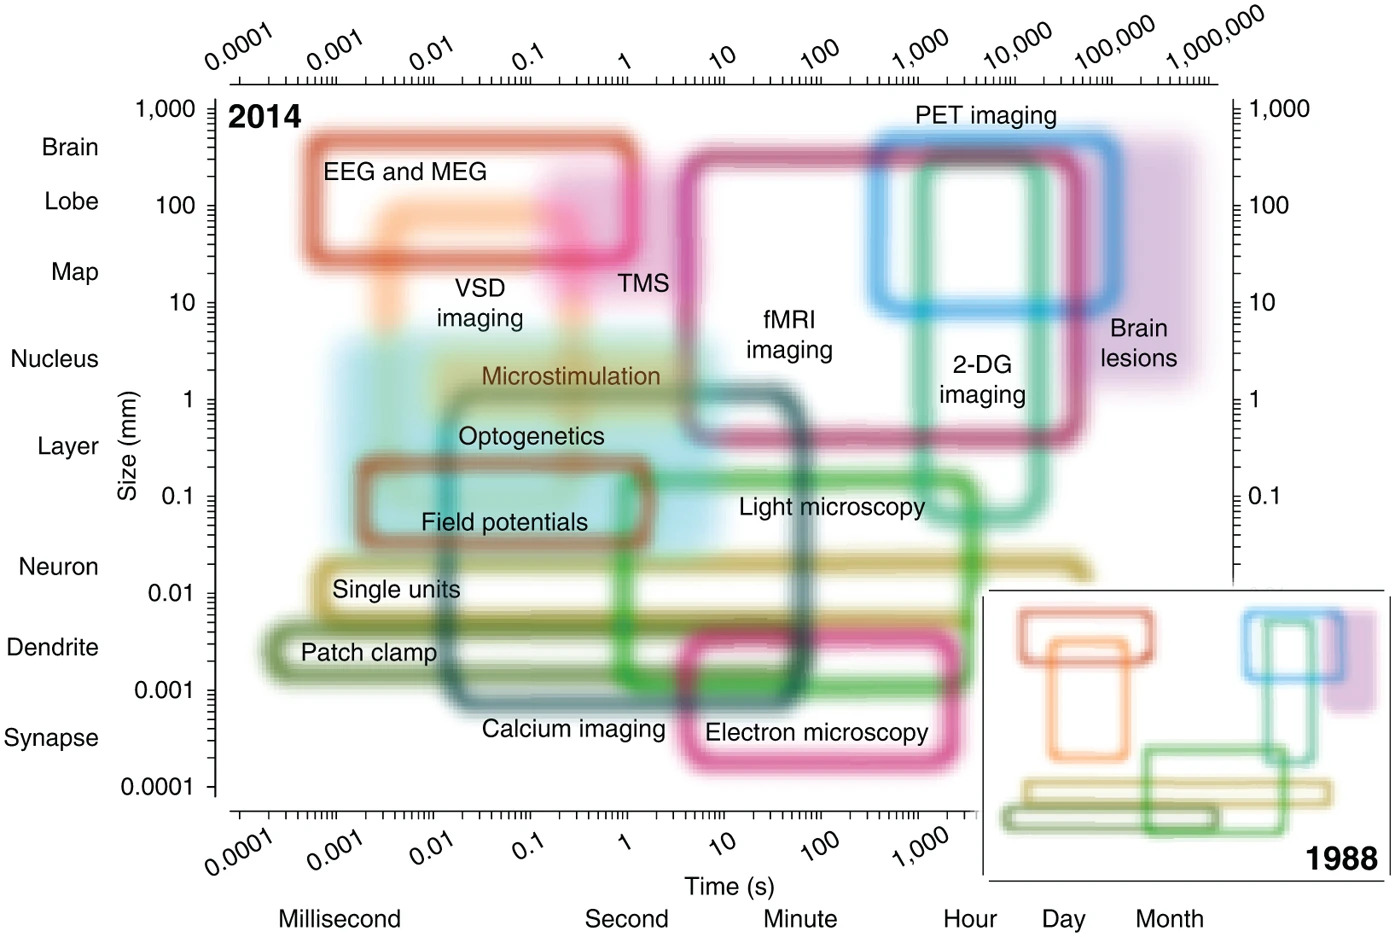
\includegraphics[width = \linewidth]{gfx/sejnowski2014pbd_fig1.jpg}
  \caption{\textbf{Spatio-temporal resolution of measurement methods in neuroscience}\\
    Demonstrate the spatial and temporal resolution of measurement methods being used in neuroscience
    (up to 2014).
    Each box depict the spatial (y-axis) and temporal (x-axis) of one measurement method.
    Open regions represent measurement techniques and 
    filled regions, perturbation techniques.
    Inset, a cartoon rendition of the methods available in 1988.
    The regions allocated to each domain are somewhat arbitrary and represent the estimate of \citet{sejnowskiPuttingBigData2014}.
    Abbreviations used in the figure:
    EEG, electroencephalography;
    MEG, magnetoencephalography;
    PET, positron emission tomography;
    VSD, voltage-sensitive dye;
    TMS, transcranial magnetic stimulation; 
    2-DG, 2-deoxyglucose.
    Figure is adopted from \citet{sejnowskiPuttingBigData2014} with permission.}
  \label{fig:measureScale}
\end{figure}
For instance, it can be spike trains from individual neurons, 
field potentials generated by small or large population of neurons or hemodynamic signals from the whole brain.
Our novel development for bridging scales pertains to the relationship between,
spiking activity
Local Field Potentials (LFPs) and 
Blood-Oxygen-Level Dependent (BOLD) signals.


A number of tools have  already been developed and applied to neural data, and they
gave us insight into the relationship between brain activity in different scales.
Here we mention very briefly a subset of such methods that are related to novel development that we introduce in the next section.


The relationship between spiking activity and LFP has been studied extensively in the context of mechanisms for coordination by oscillation in the brain.
Indeed, this was one of the examples briefly discussed in \autoref{sec:necess-invest-across} to motivate understanding cross-scale relationships.
Various techniques has been developed for investigating the relationship between spiking activity and LFP
\citep{zeitlerAssessingNeuronalCoherence2006,ashidaProcessingPhaseLockedSpikes2010,vinckPairwisePhaseConsistency2010,vinckImprovedMeasuresPhasecoupling2012,jiangMeasuringDirectionalityNeuronal2015,liUnbiasedRobustQuantification2016,zareiIntroducingComprehensiveFramework2018}.
Most of the approaches for investigating the spike-LFP coupling are restricted to pairwise first-order statistics of spike-LFP interactions.
Given the various experimental advances, there is a growing need for conceptual and methodological frameworks to investigate this relationship in multi-variate settings
(see further elaboration in \autoref{sec:relat-betw-micro}).


Another line of research pertaining to cross-scale relationships,
is investigating the relationship between LFP and fMRI BOLD signals.
In this branch,
extensive research has been done toward understanding the neural correlate
or neural activity underlying the BOLD signal
\cite{logothetisNeurophysiologicalInvestigationBasis2001,logothetisUnderpinningsBOLDFunctional2003,logothetisWhatWeCan2008,goenseNeurophysiologyBOLDFMRI2008a,zaldivarDopamineinducedDissociationBOLD2014}.
Methods used for exploring the relationship between these signals were
conventional correlation analsysis \cite{logothetisNeurophysiologicalInvestigationBasis2001},
system identification \cite{logothetisNeurophysiologicalInvestigationBasis2001},
Canonical Correlation Analysis (CCA) and its time-resolved kernelized version \cite{biessmannTemporalKernelCCA2009,murayamaRelationshipNeuralHemodynamic2010}.
Certainly, the mentioned investigation shed light on the basic nature of the coupling between LFP and fMRI BOLD, but more developments needed to get into functionally relevant couplings.


Mentioned developments construct the foundations and moreover led to important methodologies for addressing questions concerning functional implications of investigating the relationship between LFP and BOLD fMRI.
Along the same line of developments, Neural-Event-Triggered (NET) fMRI was also introduced recently. 
In NET-fMRI, characteristics neural activities of such as Sharp Wave-Ripple (SWR) are used as events to align and average the time course of large-scale brain activity to extract the global signature of the given events.
Indeed, ripple-triggered activities in macaque monkeys revealed important large-scale coordination involved in the process of memory consolidation \cite{logothetisHippocampalCorticalInteraction2012}.

NET-fMRI can be a very informative methodology if the \emph{event} is already well-defined.
Nevertheless, there are very few such well-characterized neural activity like SWR.
Therefore, we need novel methodologies to detect and characterize such distinct neural activities
(see further elaboration in \autoref{sec:relat-betw-meso}).


\section{Need for new tools for investigating cross-scale relationships} \label{sec:need-new-tools}

As was motivated in the previous section (\autoref{sec:avail-tools-invest}),
novel methodologies are needed for investigating the brain dynamics across the scale.
LFPs are signals at meso-scale  \cite{liljenstroemMesoscopicBrainDynamics2012}, 
which is an intermediate scale between micro- and macro-scale,
and they reflect a mesoscopic picture of the brain dynamics.
LFPs result from the superposition of the electric potentials generated by ionic currents flowing across the membranes of the cells located close to the tip of recording electrodes.
The LFP reflects neural cooperation due to the anisotropic cytoarchitecture of most brain regions,
allowing the summation of the extracellular currents resulting from the activity of neighboring cells and potentially remote populations. 
As such, a number of subthreshold integrative processes 
(\ie modifying the neurons' internal state without necessarily triggering spikes) 
contribute to the LFP signal
\cite{buzsakiOriginExtracellularFields2012,liljenstroemMesoscopicBrainDynamics2012,einevollModellingAnalysisLocal2013,herrerasLocalFieldPotentials2016,pesaranInvestigatingLargescaleBrain2018}.
As LFPs are rich and intermediary signals, they can be a pivotal point for bridging the scales. 
We can better illustrate the importance of LFP for cross-scale analysis with an example.
In LFPs, certain characteristics of neural activities, like
SWRs are detectable.
Interestingly, SWRs occur concurrently with well-coordinated activity at smaller scales (neurons and population of neurons),
and as well as a larger scale (entire brain).
For the connection to smaller scales (microscopic scale) various studies suggest SWRs emerge in the CA1 mainly due to afferent CA2- and CA3-ensemble \emph{synchronous} discharges \citep{csicsvariEnsemblePatternsHippocampal2000,csicsvariEnsemblePatternsHippocampal2000,olivaRoleHippocampalCA22016}.
For the larger scale (macroscopic scale), as briefly mentioned earlier, concurrent recording of BOLD signal of the entire brain and SWRs,
demonstrate large scale coordination of entire brain activity during SWRs \citep{logothetisHippocampalCorticalInteraction2012}.

Detecting characteristic activities like SWRs and finding such relationships across
scales (exemplified in the previous paragraph) was the result of years of experimental work and exploration in the data.
Developing new tools that allow us to find such characteristic
patterns (like SWRs) in an unsupervised fashion and finding their
relationship to measurement at other scales
[\eg with synchronization measures and NET-fMRI]
can be of paramount importance.

Based on the ideas and motivation elaborated above, we first focus on tools that allow us to explore
the relationship between spikes and LFPs (\autoref{sec:relat-betw-micro})
and then, a method for the detection of neural events in an unsupervised fashion (\autoref{sec:relat-betw-meso}).


\subsection{Tools to explore micro-meso relationsips}\label{sec:relat-betw-micro}
A prominent example of the relationship between micro- and meso-scale activity in the brain is the spike-field coupling.
Apart from its importance from the perspective discussed in \autoref{sec:necess-invest-across},
the synchronization between spiking activity and the phase of particular rhythms of LFP has been used as an important marker to reason about the underlying cooperative network mechanisms.
Nevertheless, there is not yet a systematic way to extract the coupling information from the largely multi-variate data available to state-of-the-art recording techniques
\cite{dickeySingleUnitStabilityUsing2009,junFullyIntegratedSilicon2017a,juavinettChronicallyImplantedNeuropixels2019}
with hundreds or even thousands of recording sites
\cite{pesaranInvestigatingLargescaleBrain2018,junFullyIntegratedSilicon2017a,buzsakiLargescaleRecordingNeuronal2004,fukushimaStudyingBrainFunctions2015}. 
We developed a multi-variate extension of phase-locking analysis 
and a statistical testing framework to assess the significance of the coupling strength.
With our method (which we call Generalized Phase Locking Analysis -- GPLA),
we can quantify, characterize, and statistically assess the interactions between population-level spiking activity and mesoscopic network dynamics (such as global oscillations and traveling waves).

We demonstrate the capability of the GPLA by applying the method to various simulated and experimental datasets.
For instance, the application of the method on simulation of hippocampal SWR can reveal various characteristics of hippocampal circuitry with minimal prior knowledge.
GPLA reveals CA1 and CA3 neurons are all coupled to the field activity in the gamma and ripple band
(in line with experimental and simulation results
\cite{buzsakiHighfrequencyNetworkOscillation1992,ramirez-villegasDissectingSynapseFrequencyDependent2018}),
suggesting this rhythm may support communication between CA1 and CA3 sub-fields during memory trace replay. 
Furthermore, it also allows us to tease apart the involved populations and provide hint on the communication flow from CA3 to CA1 based on label-free spike timing and LFP.
As another example, the application of the method on the experimental recordings from Prefrontal Cortex (PFC) suggests a non-trivial coupling between spiking activity and LFP traveling waves in this region of the PFC.
Assuming LFPs mostly reflect local and distal input post-synaptic currents to the underlying neural population,
analysis based on the GPLA accompanied by neural field simulations suggest that a connectivity structure consists of long excitatory horizontal connections and strong local recurrent inhibition as a plausible speculations for these PFC recordings
(in line with previous modeling and experimental studies \cite{safaviNonmonotonicSpatialStructure2018,sherfeyFlexibleResonancePrefrontal2018,sherfeyPrefrontalOscillationsModulate2020a}.

Notably,
an important component of our methodological contribution for investigating the relationship between micro- and meso-scale activity is the theoretical significance test for GPLA. 
We describe the theoretical foundation of the test in \citet{safaviUncoveringOrganizationNeural2023}
(\seealso, \nameref{cha:paper-5})
and the necessary development for practical applications on neural data
is described in \citet{safaviUncoveringOrganizationNeural2023}
% \shs{cite GPLA paper}
(\seealso, \nameref{cha:paper-gpla}).
In our theoretical investigation, we derive analytically the asymptotic distribution of Phase-Locking Value
(a uni-variate coupling statistics which is conventionally used for quantifying spike-LFP coupling),
which follows a Gaussian distribution.
The implication of these results for neural data is,
whitening of LFPs and normalization by the square root of the spike rate is necessary for the applicability of our theoretical results on neural data.
The asymptotic distribution for the uni-variate coupling was key for the development of the statistical test for the multivariate version of phase-locking analysis.
Based on Gaussianity of the uni-variate measure and random matrix theory we could derive the theoretical null distribution for the singular values of a matrix containing all pairwise coupling
that we call the coupling matrix.
Consequently, we show that singular values of such matrices converge to a
Marchenko-Pastur distribution
\citep{marcenkoDistributionEigenvaluesSets1967a}.
\footnote{\citet{marcenkoDistributionEigenvaluesSets1967a} in not
  written in English, but is the original publication.
  The reader can refer to \citet[Chapter
  2]{andersonIntroductionRandomMatrices2010} instead.}
This is a well-established asymptotic behavior in random matrix theory for matrices with independent normally distributed entries \cite{andersonIntroductionRandomMatrices2010}. 
The key is Marchenko-Pastur distribution has an upper bound, meaning that, 
under the null condition (no coupling between spike and LFP) largest singular value of the coupling matrix should not exceed this upper limit. 
If the singular values resulting from data are larger than this upper limit, 
then there is significant coupling between the population spikes and the multi-channel LFPs.
Developing a theoretical test is of paramount importance considering the constantly increasing dimensionality of modern recording techniques. 
\subsection{Tools to explore meso-macro relationsips}\label{sec:relat-betw-meso}

As pointed out in \autoref{sec:need-new-tools}, 
it is important to develop tools that allow us to find characteristic patterns of LFPs (such as SWRs) in an unsupervised fashion.
Such patterns are potentially very special, in the sense that,
they provide us a time window that meso-scale dynamics is closely related micro and macro scale dynamics.
In fact, this is of paramount importance for bridging the brain activity in different scales.

We developed an unsupervised methodology based on Non-negative Matrix Factorization (NMF) and dictionary learning to detect transient cooperative activities in a single channel LFP
(see \nameref{cha:paper-besserve2020ned} for more details).
Such activities were also introduced as \emph{neural events} in previous studies \cite{logothetisHippocampalCorticalInteraction2012,logothetisNeuralEventTriggeredFMRILargescale2014,ramirez-villegasDiversitySharpwaverippleLFP2015}.
With this method, is not only possible to detect well-established characteristic patterns such as sharp wave-ripples,
but also new characteristic neural activities that have not been identified and studied before.
We demonstrate the capability of our method by identifying neural events in Hippocampus and LGN and also and explored their brain-wide \emph{macro-scale} signatures using concurrent fMRI recordings from anesthetized monkey.
The result suggest that, similar to the previous study of \citet{logothetisHippocampalCorticalInteraction2012} that was focused on sharp wave-ripples,
the identified events in Hippocampus and LGN reflect a large scale coordinated dynamics,
namely a competition between cortical and subcortical regions.

Furthermore, neural events can also be informative for exploring micro-scale and meso-scale relationships.
By exploiting a simulation of thalamocortical circuitry  developed by \citet{costaThalamocorticalNeuralMass2016},
we demonstrate that such events have the potential of even relating meso-scale dynamics to \emph{micro-scale} dynamic, even at the cellular level.
With our methodology we identified different kinds of spindles in the activity of the thalamus module of the simulation (indeed, this is another demonstration for the capability of the method),
and demonstrate that different events co-occur with a characteristic activity pattern in cellular variables (such as membrane potentials and ionic currents) of the simulation.

%%% Local Variables:
%%% mode: latex
%%% TeX-master: "../phdThesis_csb"
%%% End:
